\documentclass[11pt]{article}
\usepackage{graphicx}
\parindent=.25in
\parskip=2ex

\title{APC/AST 523 Final Project : Zeus 2D}
\author{Evan Yerger and Valentin Skoutnev}

\begin{document}
\pagestyle{empty}

\maketitle

\def\normalbaselines{\baselineskip20pt \lineskip3pt \lineskiplimit3pt}

\def\mapright{\smash{\mathop{\longrightarrow}}}
\def\mapincl{\smash{\mathop{\hookrightarrow}}}
\def\mapup{\Big\uparrow}
\def\mapdown{\Big\downarrow}
\def\mapdowneq{\Big\parallel}

\def\Mapright#1{\smash{\mathop{\longrightarrow}\limits^{#1}}}
\def\Mapincl#1{\smash{\mathop{\hookrightarrow}\limits^{#1}}}
\def\Mapup#1{\Big\uparrow\rlap{$\vcenter{\hbox{$\scriptstyle#1$}}$}}
\def\Mapdown#1{\Big\downarrow\rlap{$\vcenter{\hbox{$\scriptstyle#1$}}$}}
\def\Mapdowneq#1{\Big\parallel\rlap{$\vcenter{\hbox{$\scriptstyle#1$}}$}}

\section{Overview}
This project attempted to lay the foundation for a 2D simulation of the MRI instability in astrophysical acceretion disks. Our goal was to complete the hydrodynamic algorithms and tests for the MHD equations with no electric or magnetic fields. We closely followed Stone and Norman "ZEUS-2D: A radiation magnetohydrodynamics code for astrophysical flows in two space dimensions. I-The hydrodynamic algorithms and tests" (1992). The code is written in C++ and plotted using Python's Matplotlib. We were able to implement hydrodynamic algorithms that mildy successfully pass a simple uniform advection test and the Sod shock-tube problem. However, there is still much room for improvement in using higher order interpolation methods, incorporating self gravity, and exterminating stray bugs.

\section{The Physical Setup and Equations}
The MHD equations with out electric and magnetic terms are simply the equations of hydrodynamics. The domain of these equations in our program is a 2D cartesian mesh with double periodic boundary conditions. Fluid equations are a reasonable approximation to real systems when the mean free path of particles compromising the fluid is much smaller than the length scale of the fluctions of macroscopic variables describing the fluid. Systems that fall under this category include most gases at STP and hopefully regions of an  acceretion disk around its host body.
    
    The hydrodynamic can be arrived at by taking moments of the Boltzmann equation for a fluid and closing the system with an equation state relating the pressure to the density and energy. This should be equivalant to doing the same procedure for the kinetic equations for different plasma species to obtain the MHD equations and then setting all electric and magnetic fields to zero. The set of hydrodynamic equations are: $$\frac{D\rho}{Dt}+\rho \nabla \cdotp v=0 \eqno({\bf 1})$$ $$\rho \frac{Dv}{Dt}=- \nabla p -\rho\nabla \phi \eqno({\bf 2})$$ $$\rho\frac{D}{Dt}(\frac{e}{\rho})=-p \nabla \cdotp v \eqno({\bf 3})$$

where $\frac{D}{Dt}=\frac{\partial}{\partial t}+v \cdotp \nabla$ is the comoving derivative. $\phi$ is determined from the Poission equation for gravity: $$\nabla^2 \phi=4\pi G \rho \eqno({\bf 4})$$
  
\section{Numerical Methods}
For each time interval, updating the dependent variables is done using the operator splitting procedure. The splitting is done in two steps, the source and transport steps which update equations in the following two groups:

Source: 
$$ \rho \frac{\partial v}{\partial t}=-\nabla p -\rho\nabla \phi -\nabla \cdotp Q \eqno({\bf 5})$$
$$ \frac{\partial e}{\partial t}=-p\nabla \cdot v -Q:\nabla v \eqno({\bf 6})$$

Transport: 
$$ \frac{d }{d t} \int_v \rho dV=-\int_{dV} \rho(v-v_g)dS \eqno({\bf 7})$$
$$ \frac{d }{d t} \int_v \rho v dV=-\int_{dV} \rho v(v-v_g)dS \eqno({\bf 8})$$
$$ \frac{d }{d t} \int_v e dV=-\int_{dV} e(v-v_g)dS \eqno({\bf 9})$$

$v_g$ here is the grid velocity which we take to be a constant. Also a viscous term has been added in the source term that was not in the true equations. This term is added for the purpose of dissipating unphysical effects on shock boundaries where the finite difference method breaks down. The transport step uses an intergral form because this allows the numerical method to conserve the total quantity of the advected variables to within round off error.
\subsection{Source Step}
The source step uses finite differences to compute new dependent variables. We will not write out all the numerical steps in their gory detail because they are written out in generality in Stone and Norman. We implemented their steps for cartesian coordinates. The source step is split into three parts. The first part updates the velocity due to the pressure gradients and graviational forces as shown above. The second step computes the viscosity terms. The third step computes the compressional heating term which updates the internal energy. As an example, an update for the x velocity in the first substep looks like:

$$\frac{{v_x}_{i,j}^{n+1}-{v_x}_{i,j}^{n}}{\Delta t}=-\frac{p_{i,j}^{n}-p_{i-1,j}^{n}}{\Delta x(\rho_{i,j}-\rho_{i-1,j})/2}-\frac{\phi_{i,j}^{n}-\phi_{i-1,j}^{n}}{\Delta x} \eqno({\bf 10})$$

where pressure is computed from the equation state $p=(\gamma -1)e$ for an ideal gas. 
\subsection{Transport Step}
The transport step uses finite differencing to advect the dependent variables (density, energy, and x,y,z momenta) as quantities that live inside the cell volumes. The rate of change of a quantity living in a cell volume is equal to the flux of the variable out of the cell surface. In two dimensions, the advection is done in two steps, one for each direction. The step first computes fluxes in the x direction in the entire domain using upwinded values of the dependent variables. Then these x fluxes are used to compute partially updated values of the dependent variables. Computation of the fluxes in the y direction in the entire domain then uses the upwinded value of the partially updated dependent variables. The final dependent variables are then updated using these y fluxes. 

We again don't write out the full numerical steps since they are in Stone and Norman. We adapt their technique for cartesian coordinates. As an example, updating the density looks like:

$$Fx_{i,j}=\rho_{i,j}^*({v_x}_{i,j}-v_g)dy \eqno({\bf 11})$$
$$\frac{{\rho_{partial}}_{i,j}-\rho_{i,j}}{\Delta t}=Fx_{i,j}-Fx_{i+1,j} \eqno({\bf 12})$$
$$Fy_{i,j}={\rho_{partial}}_{i,j}^*({v_y}_{i,j}-v_g)dy \eqno({\bf 13})$$
$$\frac{{\rho_{new}}_{i,j}-{\rho_{partial}}_{i,j}}{\Delta t}=Fy_{i,j}-Fy_{i,j+1} \eqno({\bf 14})$$
where $q_{i,j}^*$ means the interpolated upwind value of the $q$ variable to the cell surface.

By computing fluxes in the entire domain before using them, one is able to conserve the dependent variable to numerical precision since the sum of all the fluxes is equal to the flux out of the boundary of the domain. The interpolation upwinded method that we currently implement is the 1st order Donor Cell method. We plan to incorporate the Van Leer 2nd order method in the future.

\subsection{Poisson Solver}
Since we only use periodic boundary conditions we decided to use the Fourier series method to solve Possion's equation for $\phi$. The Poisson solver first Fourier transforms the density $\rho$. Then the Fourier transformed $\hat{\phi}$ is computed by the solving the Fourier transformed version of the Poisson equation: $$\hat{\phi}=\frac{\Delta x^2 \hat{\rho}}{2(cos(2\pi i/N_x)+cos(2\pi j/N_y)-2)}$$ Finally, $\phi$ is obtained by taking the inverse Fourier transform of $\hat{\phi}$.  

\section{Code Structure}
The program on a high level is run from $zeus\_main.cpp$. We wrote several helper classes to help keep track of time keeping (Timekeeper class), accessing arrays (Grid class), and program constants (Constants Class). Overall, $zeus\_main.cpp$ first initializes the Timekeeper, Constants, and Grid objects (which intializes all the grids we need for the source and tranport steps). Then the main function runs the time iteration. Each time step calculates $\Delta t$ using Timekeeper, then calls the poission solver (not yet incorporated), then calls the source step, and then calls the transport step, and lastly updates boundary conditions before starting over at the next time step. At the end of the entire computation it destructs all allocated memory. 

We now describe in more detail our three classes followed by the poisson solver, source step, transport step, boundary conditions, and data I/O.
\subsection{TimeKeeper class}
The Timekeeper class (in $timestep.cpp$) has one primary function: compute the $\Delta t$ for each step such that the CFL condition is satisfied in all orthogonal directions. It also keeps track of total time elapsed. As done in Zeus 2D, at the beginning of each time iteration Timekeeper takes the maximum over all grid cells of $\frac{1}{t_{max}}=max_{grid cells}(\frac{1}{(\delta t_1)^2}+\frac{1}{(\delta t_2)^2}+\frac{1}{(\delta t_3)^2}+\frac{1}{(\delta t_4)^2})^{\frac{1}{2}}$ and sets $\Delta t=C_o *t_{max}$ where $C_o$ is the safety number (Courant number). $\delta t_1$ is the minimum sound speed crossing time across a cell, $\delta t_2$ is the minimum sound flow speed crossing time across a cell in the x direction, $\delta t_3$ is the minimum flow speed crossing time across a cell in the y direction, and $\delta t_4$ is the minimum diffusion time across a cell. 
\subsection{Constants class}
The Constants class (in $constants.cpp$) simply holds the constants used throughout the program, most of which are initialized at the very beginning. The most important constants include the number of active grid cells in the x and y directions ($N_x$ and $N_y$), the size of the spacings ($dx$, $dy$, $dz$), the number of ghosts cells (2), the value of $\gamma$ (by default set to monotonic gas value $\frac{5}{3}$), and the safety factor $C_o$ (by default $C_o=.5$).
\subsection{Grid class}
The Grid class (in $grids.cpp$) is the most important one.  Grid stores the current values of the pressure, density, energy, x,y,z velocities, and potential. Grid also has several helper functions such as initializing and detroying arrays and taking finite differences of arrays in a given direction. This approach to storing arrays was chosen because for all of our functions that operate on the dependent variables we can simply pass a pointer to our Grid object to each function and then retrieve what we need from Grid. Modifiying and debugging code with this approach is vastly easier and more flexible than if we were to hard code which arrays to pass into which functions.
\subsection{Poisson Solver}
We numerically implement the method described in the {\bf \it Numerical Methods} section. To compute Fourier transforms we use the FFTW library. FFTW reference: Matteo Frigo and Steven G. Johnson, "The Design and Implementation of FFTW3," Proceedings of the IEEE 93 (2), 216–231 (2005).
\subsection{Source Step}
The source step (in $source.cpp$) is fairly straight forward and is done as described in the {\bf \it Numerical Methods} section. $source.cpp$ has a main function $source\_step()$ and several helper functions. Each substep has its own function for the X and Y direction as needed that gets called in $source\_step()$. This makes the main source step function easy to read and makes the overall step modular and thus easy to modify or debug. For reference, our commented $source\_step()$ function is shown below:

\begin{verbatim}
void source_step(Consts* c, Grid* g, double dt)
{
  //   calculate pressure from internal energy
  pressure(c, g, c->gamma-1);

  //   First substep
  subOneX(c, g, dt);
  subOneY(c, g, dt);

  //   Second substep
  subTwoQ(c, g, dt);
  subTwoVVE(c, g, dt);

  //   Third substep
  subThree(c, g, dt);

  //   Update old velocities in Grid g with newly computed ones
  replaceV(c, g);
}

\end{verbatim}
\subsection{Transport Step}
The transport step (in $transport.cpp$) ended up having roughly 5 functions to carefully compute each transport substep for each of the 5 advected variables for a total of roughly 25 functions. The transport step calculates interpolated values of every dependent variable and stores them in temporary arrays for later use in the calculation of the fluxes. Then the fluxes are computed using separate functions for each variable. Finally, each variable is updated using these fluxes via separate functions. This is done separately in the X and Y directions. Moreover, each temporary array had to have its boundary conditions updated right after it was computed.

The main function $transport\_step()$ that does all the high level computation organization is found in $transport.cpp$.

\subsection{Boundary Conditions}
The boundary conditions (in $bcs.cpp$) are updated via 4 functions for the left, right, bottom, and top rows of ghost cells (periodicL(), periodicR()...). Each function updates the respective 2 rows or columns of ghosts cells of all the dependent variables that live in Grid g. For example, for periodicL(), the far right 2 columns of the active grid are copied into the 2 columns of ghost cells on the left. The 4x4 corners are also updated in this file.     

\subsection{Data I/O}
Running a simulation requires creating a simulation folder. This folder contains files for each dependent variable that store the initial conditions. There is also a general file that stores important simulation constants such as grid size and run time. Our test cases are setup by creating a test simulation folder. 
    
    For output we are able to data dump at arbitary time intervals into the respective dependent variable folders to a create a time sequence of simulation grids for each variable. The output code also stores a general simulation file so that the simulation can be picked up again later. Overall, we can easily load and save simlulations. This code is primarily in $io.cpp$.
    
    Plotting is done in $analysis.py$ using matplotlib.

\section{Test and Results}
\subsection{Overview of Progress}

    All the aforementioned parts of the program have been coded. Our program flow control is fully functional. This part took much longer than expected. Flow control includes loading/saving simulations, time keeping, calling source/transport substeps, and updating boundary conditions. The source and transport steps seem to be working properly. Because of variarious features in our tests we still might have minor bugs find and correct. However, the use of the donor cell method renders any current simulations to be only of qualitative interest.

The first test was that of the most simple scenario: advection of a contact discontinuity. We set up a uniform flow field and square well density profile which advects across the grid. The second test was the Sod Shock Tube Test as described in Stone and Norman.

\subsection{Contact Discontinuity Advection Test}
We set up a uniform flow field with x and y velocities equal to 1. The density profile is that of a a square well. The density is 2 everywhere except at x=1 where the density is 1. We allow the program to run for a short time and see how well the contact discontinuity advects. Ideally, the profile should remain unchanged and drift to the right. We plot below the cross sections of the density, energy density, and x velocity at the beginning and end of the run:
\begin{figure}[h]
  \includegraphics[width=6cm,height=4cm]{d_0adv.png}
    \includegraphics[width=6cm,height=4cm]{d_10adv.png}
\end{figure}
\begin{figure}[h]
  \includegraphics[width=6cm,height=4cm]{e_density_0adv.png}
    \includegraphics[width=6cm,height=4cm]{e_density_10adv.png}
\end{figure}
\begin{figure}[h]
  \includegraphics[width=6cm,height=4cm]{v_1_0adv.png}
    \includegraphics[width=6cm,height=4cm]{v_1_10adv.png}
\end{figure}
\clearpage

We can clearly see that the donor cell method quickly smears out the originally sharp density profile to a depth of .08 and width of roughly 20 when it originally began with a depth of 1 and width of 1. The pulse does symmetrically advect to the right which shows that our transport step is properly advecting. However, there is a ringing wavepacket that propogates in front of the discontinuity that technically breaks the symmetry of the pulse. 
    
    We are not sure of its origin but think that it may be due to using too low of a viscosity value relative to the method we are using (we used the viscosity value that is supposed to smear shocks of widths roughly 3 cells wide as used in Zeus 2D). Because donor cell doesn't keep a very sharp boundary at the discontinuity in the beginning, ringing is able to at first grow faster than the viscosity can suppress it and so an early wave packet is able to develope and propogate. We hope this issue goes away when we upgrade to the Van Leer method, but for now we will try increasing the viscosity. Another thought is that the current combination of numerical methods is dispersive but we have not looked into this.
\subsection{Sod shock-tube Test}
We set up initial conditions as described in Stone and Norman for the Sod shock-tube test. On half the grid the pressure and density are set to $1.0$ and on the other half the pressure is set to $0.1$ and density is $0.125$. All initial velocities are set to $0$. We allowed the program to run as for as along as our patience allowed and we plot the results below (the $dt$ started around $10^{-5}$ and then kept decreasing to very small values around $10^{-7}$ as the simulation went on). These are cross section plots of our variables:

\clearpage
\begin{figure}[h!]
  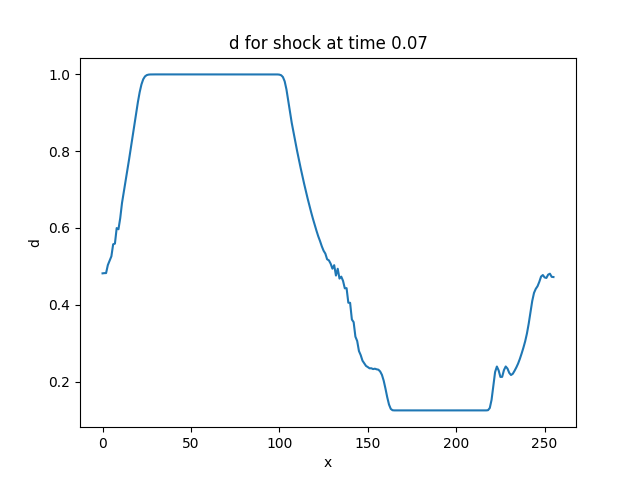
\includegraphics[width=6cm,height=4cm]{d_7.png}
    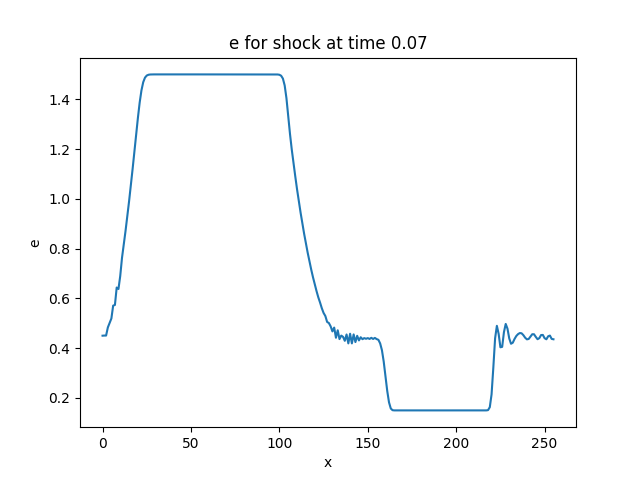
\includegraphics[width=6cm,height=4cm]{e_7.png}

\end{figure}
\begin{figure}[h]
  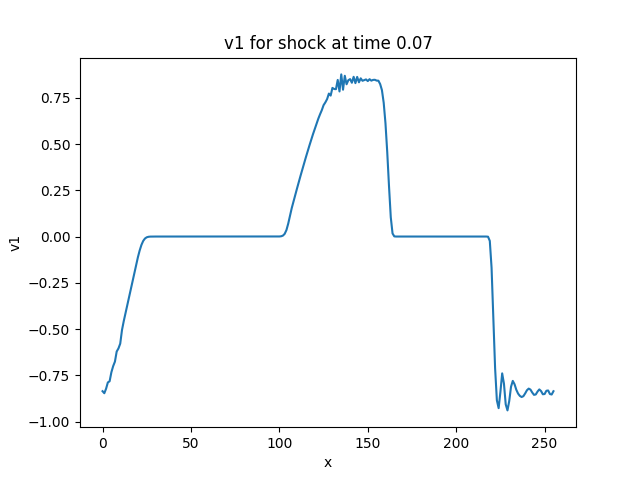
\includegraphics[width=6cm,height=4cm]{v_1_7.png}
    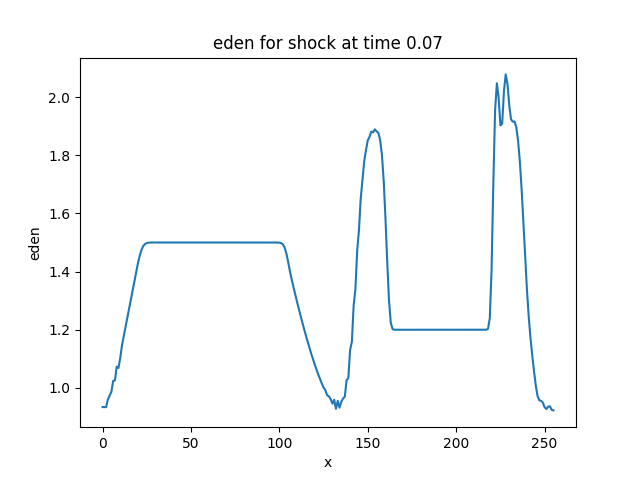
\includegraphics[width=6cm,height=4cm]{e_density_7.png}
\end{figure}
\clearpage
We compare this to the real Zeus 2D output from the paper:
 
\begin{figure}[h]
  \includegraphics[width=12cm,height=8cm]{zeusSodtest.png}
\end{figure}
\clearpage

Again the strong smearing effect of the donor cell method is very visible: we have very smoothed out corners where the Zeus 2D code remains relatively sharp 90 degree corners. However, we were excited to see that on each side of $x=190$ we qualitatively have a shock and contact discontinuity followed by a rarefaction fan. Our solution has roughly twice as many of these features as the Zeus 2D solution because we have periodic boundary conditions. In effect we roughly have a mirroring of the Zeus 2D solutions around $x=190$. 

There again is ringing around many of the features probably for the same reason explained in the advection test. The qualitative agreement gives us confidence that when we switch to a higher order interpolation method and play around more with the viscosity parameter that we will be able to get a much better physical simulation.
\clearpage
\subsection{Poission Test}
Although self gravity has not been incorporated into the code yet, we do have an independently working poission function that we have tested. Once all issues realting to pressure gradients and transport are fixed we will incorporate this function. We create two disctinct points of masses $-10/dx^2$ and compute the potential on a $1012\times 1012$ grid which we plot below. The expected $1/r$ potentials around the point masses show that the possion solver is qualitatively working correctly.
\begin{figure}[h]
  \includegraphics[width=12cm,height=9cm]{Poisson2masses.png}
\end{figure}

\subsection{Future Work}
Besides makes the code more robust and bug free, we plan to make more upgrades in the near future. We plan to change the interpolation method to the 2nd order Van Leer method and incorporate our poission solver. Minor adjustments also include swapping the order of X and Y flux calculations in order to make advection symmetric and introducing a density floor. In the long term we hope to include the M part of the MHD equations and potentially parallelize the code. This is all towards the goal of trying to simulate the 2D MRI instability and learn a lot along the way. Thank you for a very practical and interesting class.
\section{References}
Stone, J. M., and Norman, M. L. (1992). ZEUS-2D: A radiation magnetohydrodynamics code for astrophysical flows in two space dimensions. I-The hydrodynamic algorithms and tests. The Astrophysical Journal Supplement Series, 80, 753-790.

\end{document}
